\section{Evaluation}
\label{sec:eval}

This section evaluates \lang on the two workloads needed to support the paper
claim: pure-bytecode microbenchmarks that isolate kinsn opportunities, and two
production datapath case studies, Cilium and Katran. We answer four questions:
\begin{itemize}
\item \textbf{RQ1:} Does the x86 LLVM-kinsn candidate expose the expected microbenchmark speedup?
\item \textbf{RQ2:} Does a matched ARM64 ReJIT run apply kinsn sites and improve the same microbenchmark suite?
\item \textbf{RQ3:} Does \lang improve a large policy datapath, Cilium?
\item \textbf{RQ4:} Does \lang improve a packet load balancer datapath, Katran?
\end{itemize}

\subsection{RQ1: x86 Microbenchmark Signal}
\label{subsec:eval-x86-micro}

Figure~\ref{fig:eval-kinsn-micro-x86} reports the best local raw LLVM-kinsn
candidate on x86-64 KVM against the latest stock kernel eBPF baseline. Both
runs use the 29 pure-bytecode microbenchmarks from \S\ref{subsec:char-percase},
three samples, and \texttt{INNER\_REPEAT=100000}. The candidate has zero
correctness mismatches and reaches a 1.216$\times$ geomean speedup across all
29 cases. This result is useful as a selector and code-generation signal, but
we do not treat it as a matched compiler-control comparison because the kinsn
candidate and stock baseline come from different compiler/runtime
configurations.

\begin{figure*}[t]
\centering
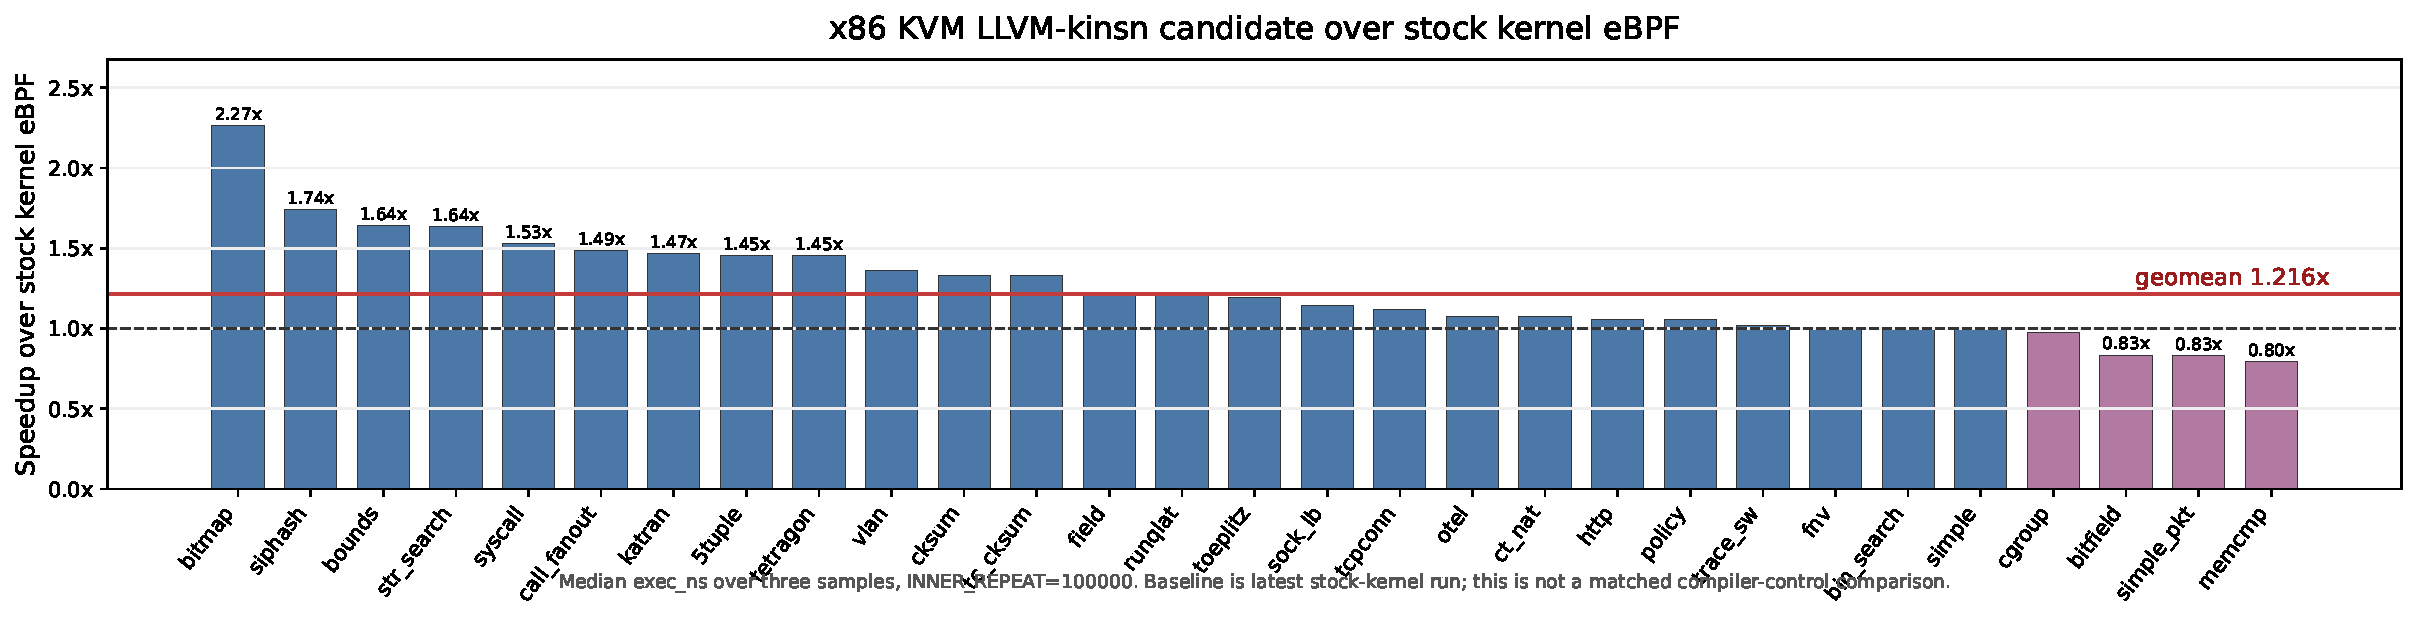
\includegraphics[width=\textwidth]{figures/sec-6-x86-kinsn-micro-best-raw-20260606.pdf}
\caption{Full per-case view for the same best local raw LLVM-kinsn candidate relative to the latest stock kernel eBPF baseline. Values use median \texttt{exec\_ns} across three samples with \texttt{INNER\_REPEAT=100000}. The geomean speedup is 1.216$\times$ over 29 cases with zero correctness mismatches, but this is not a matched compiler-control comparison.}
\label{fig:eval-kinsn-micro-x86}
\end{figure*}


\subsection{RQ2: ARM64 Matched ReJIT Microbenchmark}
\label{subsec:eval-arm64-micro}

Figure~\ref{fig:eval-kinsn-micro-arm64} reports the matched ARM64 AWS ReJIT
follow-up after fixing the selector for the pure-bytecode suite. This is the
direct comparison: the same run
contains the baseline kernel JIT measurements and the post-ReJIT measurements.
The selector applies 308/308 matched sites in the median sample and 924/924
raw matched/applied calls across the three samples. The all-29 geomean speedup
is 1.208$\times$, while the kinsn-bearing subset reaches 1.222$\times$ over
27 benchmarks with zero correctness mismatches.

\begin{table*}[t]
\centering
\scriptsize
\caption{\lang microbenchmark evaluation artifacts. The x86 row is a local LLVM-kinsn candidate against a stock-kernel baseline and is not a matched compiler-control comparison. The ARM64 row is a matched \texttt{kernel}/\texttt{kernel\_rejit} ReJIT comparison.}
\label{tab:eval-kinsn-micro}
\begin{tabular}{@{}lllccc@{}}
\toprule
Platform & Comparison & Cases & Mism. & Geomean & Sites \\
\midrule
x86-64 KVM & LLVM-kinsn candidate / stock kernel & 29 & 0 & 1.216$\times$ & n/a \\
ARM64 AWS & \texttt{kernel} / \texttt{kernel\_rejit} & 29 & 0 & 1.208$\times$ & 308/308 \\
\bottomrule
\end{tabular}
\end{table*}

\begin{figure}[t]
\centering
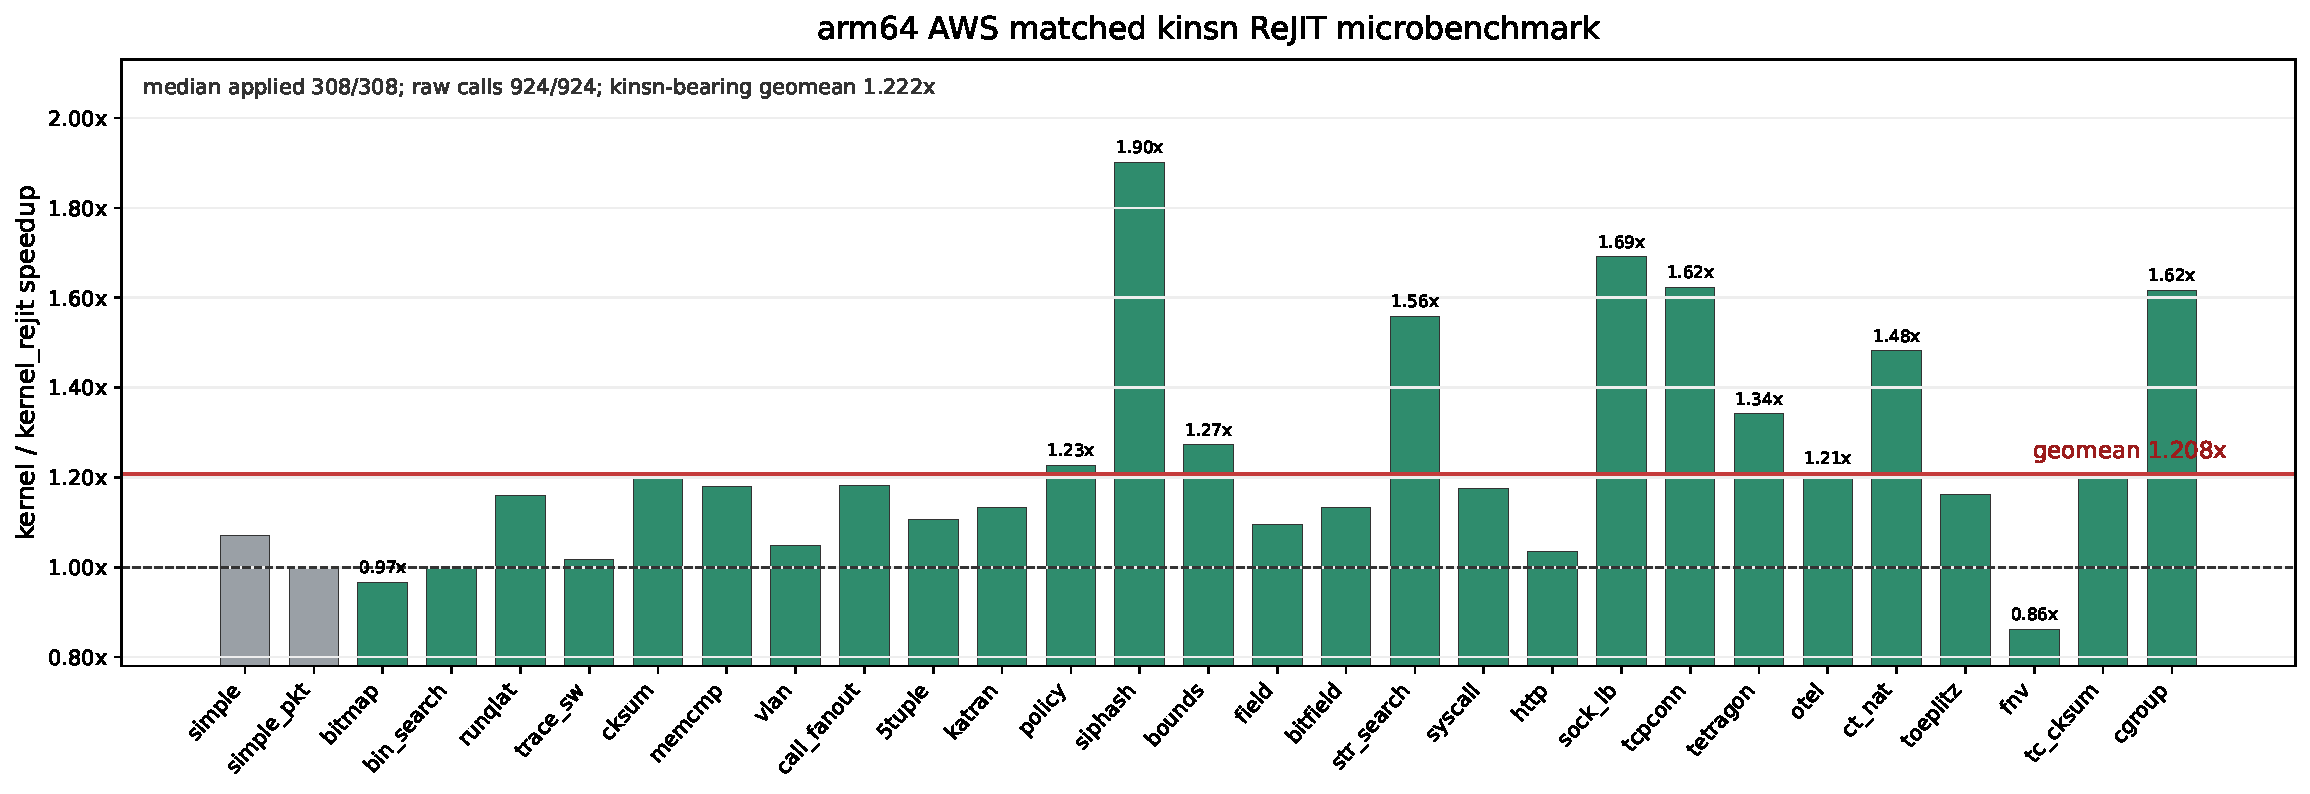
\includegraphics[width=\columnwidth]{figures/sec-6-arm64-kinsn-micro-rejit-20260606.pdf}
\caption{ARM64 AWS matched kinsn ReJIT microbenchmark follow-up for the selector-fixed pure-bytecode full suite. Bars report \texttt{kernel}/\texttt{kernel\_rejit} speedup from median \texttt{exec\_ns} across three samples. Green bars applied kinsn sites; gray bars applied none. The all-29 geomean is 1.208$\times$, and the kinsn-bearing geomean is 1.222$\times$ over 27 benchmarks.}
\label{fig:eval-kinsn-micro-arm64}
\end{figure}


\subsection{RQ3: Cilium Case Study}
\label{subsec:eval-cilium}

Cilium exercises a large packet-policy datapath with dense address arithmetic,
endian conversion, prefetch, bulk copy, and conditional-select opportunities.
The x86-64 full policy applies 4697 kinsn sites in Cilium and improves the
workload by 1.114$\times$. The retained BPF-counter population is small
(two rows), but both retained rows improve and the post-ReJIT BPF cost is
0.776$\times$ of baseline. We therefore report Cilium as a high-coverage
case study rather than as a broad fleet result.

\subsection{RQ4: Katran Case Study}
\label{subsec:eval-katran}

Katran is the cleanest production datapath for the missing-rotate story from
\S\ref{subsec:char-rotate}. On x86-64, the best local policy disables
\texttt{bulk\_memory} for Katran and keeps the scalar kinsn families that
match packet parsing and hashing: \texttt{lea}, rotate, endian fusion,
prefetch, and extract. This applies 77 sites, improves workload throughput by
1.032$\times$, and reduces BPF cost to 0.932$\times$ of baseline. On ARM64,
the conservative policy applies 21 sites, dominated by 20 rotate lowers to
\texttt{extr}, and improves workload throughput by 1.073$\times$ with BPF cost
at 0.941$\times$ of baseline.

\begin{table*}[t]
\centering
\small
\caption{Production case studies for Cilium and Katran. Workload speedup reports post-ReJIT throughput normalized to baseline. BPF cost reports post-ReJIT per-program cost normalized to baseline, so lower is better.}
\label{tab:eval-kinsn-case-studies}
\begin{tabular}{@{}llllcccl@{}}
\toprule
Case & Platform & Policy & Sites & Workload & BPF cost & Retained / W-L-T & Dominant applied families \\
\midrule
Cilium & x86-64 KVM & Full & 4697 & 1.114$\times$ & 0.776$\times$ & 2 / 2-0-0 & lea, endian, prefetch, bulk, select \\
Katran & x86-64 KVM & No bulk & 77 & 1.032$\times$ & 0.932$\times$ & 1 / 1-0-0 & lea, rotate, endian, prefetch, extract \\
Katran & ARM64 AWS & Conservative & 21 & 1.073$\times$ & 0.941$\times$ & 1 / 1-0-0 & rotate, extract \\
\bottomrule
\end{tabular}
\end{table*}

